\fancyhead[R]{{\scriptsize {\faBook\ }我们最幸福 > 顿悟}}
\chapter*{15 > 顿悟}
\addcontentsline{toc}{chapter}{\hspace{5mm}15 \textbf{>}\ \ 顿悟}
\vspace{20mm}
\begin{flushright}
	\textcolor{PinYinColor}{\EN \huge{Epiphany\\
			\ \\}}
\end{flushright}

\begin{figure}[!htbp]
	\centering
	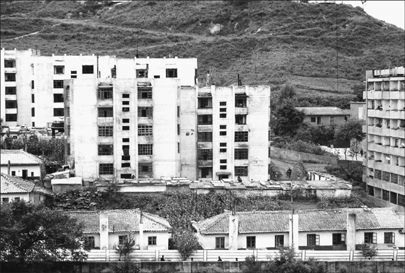
\includegraphics[width=6cm]{./Chapters/Images/15.jpg}
	\caption*{清津的住宅区}
\end{figure}

在平壤的大学里,俊相非常依赖那反复无常的邮政系统里老家的朋友、家人保持联系。除了美兰,他还固定的同几个人保持联系。他母亲也会把家里狗的一些趣闻写信告诉他。而父亲则总是要求他刻苦学习:“为了金日成,为了精心培养你的劳动党。”他总是用这样的语句作为信件的结尾。希望以此取悦那些检查信件的核查员。在寒冷的冬季,那些信件很有可能被铁路职工用于取暖御寒而烧掉了,因此俊相就可能几个月里一封信也收不到。所以,当他写给美兰的信件都石沉大海、杳无音信的时候,他一点也不奇怪。但是当十月过去了、十一月过去了、然后十二月也过去了,仍然没有她的只言词组,俊相就开始担心了。那个冬天,当一回到清津,他就装作随口闲聊一样的问他弟弟最近有没有碰到过美兰。他弟弟却不等他说完就脱口而出,“她走了!“

“走了,走去哪里?”俊相不敢相信他所听到的。关于美兰计划的行程,他没有得到一丁点的征兆。她总是会把她的任何事情都告诉自己的,不是吗?虽然在夏天的时候,她给他的回信里语气有点不好,但是那可能是因为还在嗔怪他不愿意结婚吧,他不能相信她就这样不辞而别了。他抓紧弟弟,想得知更多的消息。

“他们都走了。有传言说他们已经到了南韩。”弟弟知道的只是这么多。

他去了她家附近,想了解些更多。他先是在她家附近转悠,好像在实施监视一样;他不能靠的再近了。他觉得肚子里一阵紧似一阵;自己脖子的青筋也在狂跳。几天后,他回来了。他在多年来同美丽秘密约会时,一直等她出现的那堵墙下坐了很久。他亲眼看到,现在那间房子里住着另外一户人家。

那个假期里,还有后来的每一次回家,他都会不断的回到那间房子。仅仅是想打听些消息──除了传言,没人知道更多。他怎么这么白痴。他恨自己;他做任何事情总是犹犹豫豫,瞻前顾后,好不容易下定决心却又发现太迟了。他思前想后的,终于决定向她求婚了,而她却走了。纵观他们的感情,他总认为自己是主导方。他是男人,他年长几岁,他有大学文凭。他给她带来平壤的诗,告诉她那些她闻所未闻的小说、电影。但是到头来,她才是勇敢者,而自己却是个懦夫。当然这无人知晓,但是他心里有一种感觉──她在南韩。

该死,她居然比我早行动,他告诉自己。

实际上,美兰的动作几乎比任何人都早。

从朝鲜战争结束后,到美兰1998年10月逃亡之前,几乎半个世纪中,一共只有928名北朝鲜人逃到了南韩。对比于柏林墙屹立时,每年多达两万多东德人逃往西方,这个数字几乎可以忽略不计。

这些逃亡的北朝鲜人,大多是外交官或者在国外旅行的官员。黄长烨,北朝鲜高级学者和领导人,曾经作为金正日的教授,在一次出访回国途经北京时,走进南韩驻北京大使馆。偶尔,也会有北朝鲜的士兵历经艰难险阻,穿过非军事区叛逃至南韩。还有一些渔民,则坐船前往南韩。

北朝鲜当局采取一切可能的措施锁住自己的国民。在清津和其它沿海城市,九十年代早期,就沿着海岸树立起一道围栏,防止人们乘船驶向日本。当北朝鲜人离开这个国家出公差,他们必须留下自己的配偶或者孩子作为有效的人质用以确保他们会回来。他们要逃亡者明白,自己的自由,是以至亲爱人下半辈子将永远生活在劳动营作为代价的。

形势在九十年代末发生了变化。饥荒以及中国经济状况的改变给了北朝鲜人以逃亡的动机。从边境,他们可以看到图们江那一侧沿着江堤跑着闪亮的汽车。他们用自己的眼睛可以看见,中国的生活看上去很好。

帮助美兰过江的地下网络迅速扩大他们的运营。他们不断的变换跨过图们江的线路,标记出最窄的跨越点,以及哪些守卫是可以被收买的。如果你不会游泳,你可以雇人背你过去。逃亡者的数量也急剧增加。2001年,估计有多达十万的北朝鲜人潜入中国,但是他们当中,只有很少一部分最终抵达南韩。

交易流动是双向的。北朝鲜的人逃往中国;中国的货品输进北朝鲜,货物不仅仅是食品、服装、还有书籍、杂志、甚至圣经,这在北朝鲜是非法的。中国盗版工厂生产的DVD光盘体积小、价格低廉。一个走私者一次就可以在一个小小的箱子里夹带数千张,上面再摆上一层孝敬给警卫的香烟。DVD播放机也是中国制造的,只需要二十美元就可以买上一个。通过这种方式,北朝鲜人在新经济下,私人赚取着利润。热卖的影片有《泰坦尼克》(Titanic)、《空中监狱》(Con Air)、《目击者》(Witness)等。更受欢迎的是南韩的影视剧,还有夸张的甜蜜肥皂剧。南韩的情景喜剧应当描绘的是普通工薪阶层的生活故事,但是北朝鲜人却特别关注节目里所展示的厨房家电和角色的服装。有史以来第一次,普通的北朝鲜人能看到用他们自己的语言演绎的,没有任何金日成或者金正日出现的节目。这些影碟使北朝鲜人得以一窥另一种生活方式。

然而,北朝鲜政府却指控美国和南韩将DVD影碟和书籍输入北朝鲜,阴谋颠覆北朝鲜政权。DVD小贩被逮捕,甚至以叛国罪名被处以极刑。劳动党党员也发表演说,警告人们抵制外国的文化侵蚀:

\begin{quote}
	\begin{spacing}{0.5}  %行間距倍率
		\textit{{\footnotesize
					\begin{description}
						\item[\textcolor{Gray}{\faQuoteRight}] 	我们的敌人正在用一些专门制作的材料来美化帝国主义,传播他们极其腐朽的资产阶级生活方式。假使我们让自己受这些专门制作的材料毒害,那我们的革命思想、我们的阶级意识就会丧失,我们对统帅金日成的绝对崇敬就会消散。
					\end{description}
				}}
	\end{spacing}
\end{quote}

然而在北朝鲜,藉助于书本、报纸或电影传播信息的效果远远不如人们的口口相传。那些没有手段看外国DVD影碟的人就会从其它人那里听说。然后关于邻国的富裕、科技的发达就以不可思议的程度传播着。有人说,南韩发展了一种轿车是如此的先进,只有在驾驶者先通过一种酒精测试以证明他处于清醒状态下,汽车才会启动\footnote{这不是真实的情况。},还有边界对面的普通中国农民十分富裕,以至于他们一天三顿、顿顿白米饭\footnote{这是真实的情况。}。

一个北朝鲜的士兵后来回忆,一个朋友有一把美国产的指甲钳,那个朋友很得意的向他炫耀。这个士兵用它剪了几个指甲,很是钦佩它的锋利,整洁的刀刃,并且惊叹于这个简单小东西的做工。然后,他突然心里一沉,意识到:如果北朝鲜做不了这么精细的指甲钳,它又拿什么去和美国生产的武器竞争呢?

有一个北朝鲜学生在官方媒体上展示的一张显示在罢工现场,警方拘捕前的一个南韩人的照片。照片的本意是想揭示在资本主义社会里被剥削的工人;然而适得其反的是,这个学生却注意到这个“被压迫的”工人身上穿着一件带有拉链的夹克,口袋上还别有一支圆珠笔,而这两样东西当时在北朝鲜可都是十分稀罕的奢侈品。

一个北朝鲜的海事官员于九十年代中期时待在一艘航行在黄海的船上,此时收音机碰巧收到了南韩的广播信号。那个节目是个情景喜剧,说的是两个年轻女人争抢公寓楼前一个停车位的事情。他根本理解不了一个地方怎么会有那么多车,以至于会没有地方去停车。虽然那个时候他已经三十多岁了,而且阶级也不低,但是他还从来没听说过有人有私车──就更不要提年轻女性了。因此,他猜想这个节目是一出拙劣的表演,但是反复琢磨了几天之后,他被深深的震撼了,是的,南韩肯定有很多汽车。

他几年后叛逃了,正如那个用了指甲钳的士兵和那个看到罢工照片的学生一样。

即使在最疯狂的梦境里,金医生也从来不曾设想会离开北朝鲜。并不是因为愚昧无知,也不是因为对外界没有好奇心──她非常热爱读书,很喜爱来自遥远国度的异国爱情故事──但是就她而言,北朝鲜是世界上最好的国家。为什么还要去其它地方呢?

在整个童年时期,金医生经常听父亲讲述六十年代早期逃往北朝鲜之前他在中国的悲惨生活。因此,金医生十分庆幸自己能在北朝鲜出生,更让人感激的是政府让她这样一个卑微的建筑工人的女儿免费进入医学院学习。她认为自己应该用所学,用生命来报答她的国家。这也是她期待加入劳动党的最大动力,以期能偿还自己对国家的所欠。

“如果党需要我献出生命,我就会毫不犹豫。我是如此的爱着我的祖国。”她后来这样说道。

金医生志愿担任额外的工作──党委书记的助理──在此期间,她却发现党不是这样看待她的。

在金日成去世的那个冬天,金医生的志愿工作让她不得不早上七点半就到了医院,她要赶在其它高级职员到之前,将党委书记乱糟糟的办公室整理干净,党委书记是一位五十多岁的女医生,肝病专家,通常被人们称为张书记同志。她的办公室是个小间,一面墙上按规定挂着金日成、金正日的画像,其余的墙边放满文件柜。老式带抽斗的办公桌抽屉总是关不严,因此文件会漏出来,散落在地上。然而,报纸却仔细的迭放在桌子上。报纸是不能随便扔在地上的,以免人们会踩着上面印着的金日成、金正日照片。张书记同志不太喜欢读写;她的这些事情完全都是由金医生代劳,金医生给她读《劳动新闻》和当地报纸《咸镜新闻》的社论,为她准备讲演稿子。作为回报,她很自信书记同志会作为她的入党介绍人。她甚至还大胆想象,自己有朝一日也会沿着她的轨迹,当上党委书记。

当她整理办公室的时候,金医生注意到一个木文件柜开着。此时她的好奇心占了上峰。一堆文件里,一个大信封露了出来。她打开信封,发现里面有个名单都是她认识的单位同事,他们的名字都位列于需要特别监视的栏目之下。每个名字之后还有一些评价,说明他们被怀疑的原因。大多数都是因为家庭背景──父母或者祖父母是教徒,或者是地主的子女,家里有从日本来归的朝侨,或者家有亲戚在中国。

她的名字也在这个名单里。

金医生半信半疑。整个一生,她的行为都无懈可击。她天生是个完美主义者,以极高的标准要求自己。当还是学生的时候,她的成绩就非常优秀。她总是积极参与志愿工作,参加额外的政治思想学习。她的父亲来自中国,在那里也仍然有亲戚,但是金医生和他们从未谋面,也未曾有过联系。

可能弄错了,她告诉自己。

最后,真相水落石出。张书记同志只是在敷衍她,让她干这干那,却对她入党的事情绝口不提。更糟糕的是,金医生开始怀疑她真的是被监视着。她觉得医院里那些党干部总是对她特别关注。

直到两年后,她最终确定了她的怀疑。一个国家安全特工突然来医院找她,这个人为保卫部工作,一个专门调查政治犯罪的警察部门。起先,金医生以为他来调查她父母或者同事,但是他却只问关于她的问题,她的家庭、她的工作,直到最后,他才来到重点。他此行的目的是评估她会不会叛逃。

“离开北朝鲜?”金医生愤怒了。她从来没有考虑过这样的事情。当然,她听说过有人离开的传言,但是她非常瞧不起那些在艰难行军中意志力不坚强、且背叛祖国的人。

“为什么我要离开?”她抗议道。

这个特工列举了些原因。她有亲戚在中国。她的婚姻破裂了。医院付不出工资。

“你!我们盯着你。别想跑!”他离开前恶狠狠的威胁道。

后来,她在脑子里不断的重复着这次谈话。她想的越多,就越是觉得那个保卫部的人所说的原因有道理。他把这个想法种进了她脑子,根深蒂固,她发现无法甩掉。

她在北朝鲜的生活简直糟透了。她的前夫在离婚后很快就再婚了。按照北朝鲜典型的离婚做法,她六岁大的儿子和奶奶住。根据法律和习俗,孩子属于父亲一边,也只名列父亲家的族谱上。金医生只能偶尔在周末去看看孩子,而那时她对孩子的又小又瘦感到焦虑万分。他的前夫和婆婆家里也没有太多吃的。

她吃的也好不到哪里去。其它的医生通过卖药或者做手术,特别是堕胎手术来贴补家用。而金医生没有受过这方面的培训,也不愿意做这样的事情。因此,她也只能草草的吃些病人送的食物,但是不久之后,病人也没有多少可以给的了。

金医生于1997年申请调离儿科,她实在无法忍受那些饥饿孩子的眼神。她转到了研究部门,以此希望不再接触那些将死之人,但是医院里根本没什么条件开展研究。早餐之后,医生们就一个个忙着准备晚餐,晚餐后,他们又开始发愁明天的早餐。她开始早退去山里面找些能吃的野菜。有时候她也会砍些柴去买。她的体重降至三十六公斤以下。她的乳房干瘪、月经也停了。那时候,她看上去就像个十二岁的孩子而不是个三十出头的女人。没有吃的那头几天,她饿的都想去偷一个孩子的食物。但是差不多四天过后,她也就觉得没什么了,只是有股奇怪的感觉,觉得自己的身体不是自己的。她觉得自己好像飘在空中,然后又掉下来了。她的身体已经差不多耗尽了。早上,她没有力气起床。她也不再去义务帮党书记工作了,到1998年的时候,她彻底不去上班了。她想方设法的赚钱,在市场上卖酒、卖煤。她根本不在乎荒废了在医学院学到的本领。在饥荒最严重的时刻,活下来就可以了。

在她一次去的一个市场里,她碰见了一个老朋友。她们在高中就是同学,她们是一类学生,聪明且都被认为“最有前途。”她朋友曾是个班干部。她们礼貌的寒暄了一阵,相互恭维对方看上去气色很好,虽然她们都面黄肌瘦。然后,金医生问了问她的家庭。她丈夫和亮岁的孩子就在三天前死了,她说这些的时候,好像事不关已一样。

金医生试图安慰她。

“哦,我现在好多了。要喂的嘴少了。”她告诉金医生。

金医生分不清她朋友是麻木了还是精神错乱,但是她知道如果她在北朝鲜再待下去,她也会和这个朋友一样,或者她早就死了。

在死之前,金医生的父亲给了她一个名单,上面有他在中国的亲戚的姓名和最后知道的地址。这是自杀之类的绝笔。她父亲用颤抖的手,在绝食的弥留之际写成。曾几何时,金医生觉得被这张纸条冒犯,但是最终她没有把纸条扔掉。她找出了装纸条的小铁盒子,小心的展开那张纸,看着那些名字。

“他们会帮你的。”她父亲曾说过。

金医生独自一人前往中国。她没钱雇向导或贿赂边境守卫,所以她只能依赖自己的头脑和直觉。在1999年3月,已经有很多人成功逃离,因此在一些边境城市,你可以就跨界最好的地点和时机听见一些小建议。其时严冬刚刚过去,早春的景象刚刚展现,图们江上有些江段仍然封冻着。金医生到了一处听说江面仍然可以走人的地点。每隔几米,她就向前投掷一块重石,测试冰面的厚度。至少在北朝鲜一侧,冰面还足够结实。她先把一只脚滑向前,然后是另外一只脚,动作优雅的像个芭蕾舞演员。她大概来到了江中心的时候,突然石头在一次投掷中消失在淤泥中。她也随之掉了下去,刺骨的江水一下子淹到腰部。她好像在爬一座冰山一样,手脚并用的爬了出来。

金医生挣扎的爬上江岸。她的腿包在冻硬的裤子里,完全没有了知觉。她摸索着穿过了树林,在晨曦第一缕阳光照亮天空的时候,她找到了一个小村子。她不想坐下来休息一会儿,她害怕那样会死于体温过低,但是她很清楚自己没有力气走的更远了。她只好试一试向当地居民寻求帮助。

金医生看见一条土路通往一些农舍。这些房子大多由围墙围着,前面有个铁门。她轻轻的试了试一扇门;门没有锁。她把门推开,朝里面张望。在地上,她看见一个小金属碗里面装着些吃的。她又凑近看了看,是一碗米饭,白米饭,还混了些肉在里面。金医生已经不记得自己上一次看见整碗的白米饭是什么时候的事情了。但是一碗米饭放在这干什么,就放在地上?当听见狗叫的时候,她一切都明白了。

就在此之前,她还曾有点希望中国会和北朝鲜一样的穷。她仍然愿意相信她的国家是世界上最好的地方。她珍爱一生的信仰会被证明是正确的。但是现在她面对的是眼前不可否认的痛苦事实:中国的狗吃的都比北朝鲜的医生好。
